\section{Commutativity in the Weak Queue Specification}
\label{wqueue}

To demonstrate how the strong queue interface and the corresponding commutativity of transactions prevents a scalable transactional queue implementation, we can imagine a different queue interface---a \emph{weak queue specification}---that increases commutativity of operations and transactions, and \emph{does} allow for a scalable transactional queue implementation. This interface is shown in Figure~\ref{fig:wq_interface}, and differs from the strong queue specification because a pop operation returns \texttt{void} instead of \texttt{bool}. 

\begin{figure}[t]
    \centering
    \begin{lstlisting}
                        void push(const value_type& v); 
                        void pop();                     
    \end{lstlisting}
    \caption{Weak Queue Operations Interface}
    \label{fig:wq_interface}
\end{figure}

In a non-transactional setting, calling a pop with this interface does not observe the empty status of the queue, which allows a pop to commute with all operations in all scenarios (exchanging the order of a pop and another operation would have no observable effect to the caller). With this interface, a queue can even return \texttt{void} without performing any actions, which makes the queue extremely scalable (but rather useless). 

To still have a useful transactional queue, we add an extra condition that a pop operation in a transactional setting be assigned a \texttt{true} or \texttt{false} value when its containing transaction commits. For example, a singleton transaction containing a pop will return \texttt{true} or \texttt{false} at the time of commit.
These pop operations must satisfy both the invariants of a \emph{concurrent} queue described in Section~\ref{q_spec}, as well as the invariant that, at commit time, the pops remove consecutive values off the queue. Furthermore, the pop operations cannot pop the values that were pushed within the same transaction. The invariants for a push remain the same (two pushes in the same transaction must appear consecutively in the queue).
The queue under this specification retains all the fairness properties of a concurrent queue: no value remains in the queue forever, because values are still removed in the order in which they are added. Like Schwarz~\cite{schwarz}, we see uses for this transactional queue as a buffer between producer and consumer activities, in which the exact ordering of values in the buffer is unimportant, and a transaction does not need to know exactly how many values were actually popped. Examples of valid weak queue transactional histories are shown in Table~\ref{tab:txnal_weakq_commute}.

A weak transactional queue has greater commutativity than a strong transactional one. Individual pop operations now commute with any operation, because they return \texttt{void} when called. Thus, instead of having to synchronize \emph{both} individual pop operations and the \texttt{COMMIT\_TXN} operations of transactions (as the strong transactional queue must), the weak transactional queue only needs to synchronize the \texttt{COMMIT\_TXN} operations, which now return a list of \texttt{bool} values (one for each pop operation within the transaction). This is because only \texttt{COMMIT\_TXN} operations return non-\texttt{void} values, and therefore fail to commute.
We claim that synchronizing these \texttt{COMMIT\_TXN} operations is no more difficult than synchronizing strong queue pops in a non-transactional setting: we can use the same commutativity reasoning we used to reason about commutativity between individual strong pops and pushes to reason about commutativity between weak \texttt{COMMIT\_TXN} operations. A weak \texttt{COMMIT\_TXN} operation can be broken down into a pop-group operation and a push-group operation. It is clear that a pop-group that encounters an empty queue will not commute with another pop-group or a push-group; thus, we see that a pop-group has equivalent commutativity behavior to a strong pop, and a push-group has equivalent commutativity behavior to a strong push. Indeed, performing a weak \texttt{COMMIT\_TXN} operation and performing a strong pop operation both require protected access to the queue's head and do not scale.

\begin{table}[H]
    \centering
    \singlespace
    \begin{tabular}{|l|l|}
        \hline
\multicolumn{1}{|c|}{Valid History Interleaving} & \multicolumn{1}{c|}{Serialized Forms of History}\\
        \hline
\begin{lstlisting}
// Q empty
(T1, START_TXN, ())                       
(T2, START_TXN, ())                       
(T2, Q.pop(), ())                       
(T1, Q.pop(), ())                       
(T1, Q.push(a), ())                       
(T1, Q.push(a), ())                       
(T1, COMMIT_TXN, {false})                       
(T2, COMMIT_TXN, {true/false})                       
\end{lstlisting} &
\begin{lstlisting}
// Q empty
(T1, START_TXN, ())                       
(T1, Q.pop(), ())                       
(T1, Q.push(a), ())                       
(T1, Q.push(a), ())                       
(T1, COMMIT_TXN, {false})                       
(T2, START_TXN, ())                       
(T2, Q.pop(), ())                       
(T2, COMMIT_TXN, {true})                       
 ------------------------------
// Q empty
(T2, START_TXN, ())                       
(T2, Q.pop(), ())                       
(T2, COMMIT_TXN, {false})                       
(T1, START_TXN, ())                       
(T1, Q.pop(), ())                       
(T1, Q.push(a), ())                       
(T1, Q.push(a), ())                       
(T1, COMMIT_TXN, {false})                       
\end{lstlisting}\\
\hline
\begin{lstlisting}
// Q empty
(T1, START_TXN, ())                       
(T1, Q.push(a), ())                       
(T1, Q.pop(), ())                       
(T1, Q.pop(), ())                       
(T2, Q.pop(), ())                       
(T1, Q.push(a), ())                       
(T1, COMMIT_TXN, {false, false})                       
(T2, START_TXN, ())                       
(T2, COMMIT_TXN, {true/false})                       
\end{lstlisting} &
\begin{lstlisting}
// Q empty
(T1, START_TXN, ())                       
(T1, Q.push(a), ())                       
(T1, Q.pop(), ())                       
(T1, Q.pop(), ())                       
(T1, Q.push(a), ())                       
(T1, COMMIT_TXN, {false, false})                       
(T2, START_TXN, ())                       
(T2, Q.pop(), ())                       
(T2, COMMIT_TXN, {true})                       
 ------------------------------
// Q empty
(T2, START_TXN, ())                       
(T2, Q.pop(), ())                       
(T2, COMMIT_TXN, {false})                       
(T1, START_TXN, ())                       
(T1, Q.push(a), ())                       
(T1, Q.pop(), ())                       
(T1, Q.pop(), ())                       
(T1, Q.push(a), ())                       
(T1, COMMIT_TXN, {true, false})                       
\end{lstlisting}\\
    \hline
    
    \end{tabular}
    \caption[Examples of valid weak queue transaction histories.]{Examples of valid weak queue transaction histories.}
    \label{tab:txnal_weakq_commute}
    \end{table}

To support this point, we implement an example of a weak transactional queue using the flat combining algorithm, and show that the flat combining's non-transactional synchronization mechanism for a strong pop can be used in a nearly unmodified form in order to support transactions with our weak specification.


\subsection{The Weak Transactional Flat Combining Queue}
The Weak Transactional Flat Combining Queue (WT-FCQueue) demonstrates how the flat combining technique's performance depends upon the commutativity of operations satisfying a particular queue specification in a transactional setting. It also provides support that the commutativity of operations satisfying the weak queue specification in a transactional setting is equivalent to the commutativity of operations of a non-transactional queue satisfying the strong queue specification.

This queue implements the weak transactional queue specification using \emph{LazyPops}: instead of returning \texttt{bool}, a pop will return a LazyPop. The LazyPop will be instantiated with a \texttt{true} or \texttt{false} boolean value at commit time, but prior to that time, the LazyPop's value cannot be accessed.
At commit time, our implementation performs a pop using the non-transactional flat combining \texttt{<POP>} request, and assigns the corresponding boolean return value to the corresponding LazyPop. All pushes from the transaction are also installed at commit time using the \texttt{<PUSH, write\_list>} request described earlier. We note that both pop and push requests do not need to access the queue during execution time. This allows us to minimize the number of flat combining calls: we do not need to generate additional flat combining calls during transaction execution because the queue does not need to be accessed until commit time.

Our implementation satisfies a weaker specification than the weak queue specification described above: in our implementation, pops are not guaranteed to be consecutive and a pop cannot remove a value pushed earlier in the same transaction (no \emph{read-my-writes}). However, we hypothesize that a queue that installs all pops at once---by posting, at commit time, a \texttt{<POP, num\_pops>} request that returns a list of booleans---will perform no worse than our current method of pops (or may perhaps even perform better). This is because the synchronization is still restricted to the point at which the \texttt{COMMIT\_TXN} operations occur in the history, and in both our implementation and our proposed hypothetical weak transactional flat combining implementation, concurrent access to the queue is restricted to a single thread at this point.

\subsection{Evaluation and Results}

\begin{figure}[t]
    \centering
    \boxed{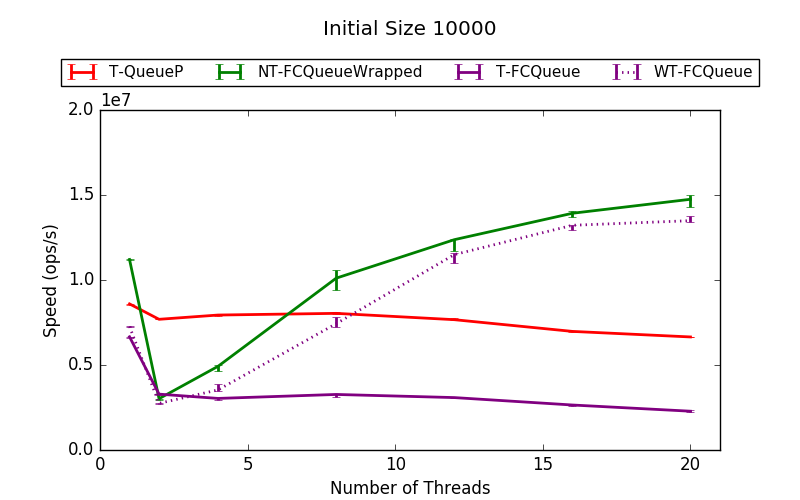
\includegraphics[width=\textwidth]{fcqueues/lpQ:RandSingleOps10000.png}}
    \caption{WT-FCQueue Performance, Multi-Thread Singletons Test}
    \label{fig:wtqs}
\end{figure}

We evaluate the weak transactional flat-combining queue on the same benchmarks described in Section~\ref{q_microbenchmarks} to compare against the strong transactional flat-combining queue (T-FCQueue), T-QueueP, and NT-FCQueueWrapped. Selected results are shown in Figure~\ref{fig:wtqs}; full results are in Appendix~\ref{app:queues}. 

While the weak transactional flat combining queue (WT-FCQueue) does not perform as well as its non-transactional counterpart, NT-FCQueue, the performance of WT-FCQueue exceeds that of the T-QueueO, the T-QueueP, and the T-FCQueue, which all provide full-transactional guarantees. We see gains in performance over the T-QueueP up to 1.5$\times$ as the number of threads accessing the queue increases to 20; the WT-FCQueue begins to outperform the T-QueueP as the number of threads increases past 7. The WT-FCQueue outperforms the T-FCQueue starting at 4 threads and achieves performance up to about 5$\times$ by 20 threads.
 
The WT-FCQueue does not experience any aborts. This is due to the flat combining algorithm, which does not require that any locks be held in the weak transactional setting in order to ensure correctness. A transaction can abort only if the result of a pop is accessed during the transaction's execution.
Because of the lack of aborts, the WT-FCQueue significantly outperforms the T-FCQueue; this demonstrates the effectiveness of the flat combining technique in the weak transactional setting. 

%We compare the WT-FCQueue against the WT-Queue to evaluate whether performance improves because we changed the queue algorithm, or whether performance improves because the weakly-transactional specification has fewer requirements than the strongly-transactional specification. The WT-Queue performs worse than all other queues because of its high abort rate (50--70\% as the number of threads increases, with 100\% of aborts occurring at commit time). This is caused by contention on the headversion and the tail version locks. While the actual pop function called during a transaction's execution is much simpler than in the T-QueueO or T-QueueP algorithms---it does not access the queue to check if the queue is empty---the installation procedure becomes more complicated; installing a pop requires instantiating all LazyPops, which more than doubles the number of cache misses of the T-QueueP. The WT-FCQueue incurs approximately 2$\times$ more cache misses than the NT-FCQueue, but is not crippled from LazyPop-caused cache misses because the flat combining algorithm optimizes for efficient cache usage. Unlike the WT-FCQueue, the WT-Queue holds a global lock during installation at commit time, aborting or delaying other transactions that attempt to commit. Thus, we see that the flat combining algorithm, and not the choice of transactional specification, is the source of the weak transactional, flat combining queue's increased performance.

Our results show significant improvements in the performance of the flat combining algorithm when satisfying the weakly-transactional queue specification compared to its performance when satisfying a strong transactional one. This demonstrates that the commutativity of operations under a queue specification in a transactional setting directly affects the effectiveness of the flat combining algorithm. We argue that the modifications to provide transactional guarantees with our strong queue operation interface critically impair the performance of the flat combining algorithm, and that these modifications cannot be avoided. Thus, scalable performance of a strong flat combining queue is unlikely to be achievable in a transactional setting.
